\section{Model}

\subsection{词嵌入层}
如何有效的表示文本是NLP领域最基础也是最重要的问题之一,早期的表示文本的方式有one-hot形式或词袋模型。
one-hot也称独热编码,将单词表示为一个只有0和1两个值的向量,大小和语料库中词典的大小相同,每一个单词都有自己的编号,
对应于自己编号的位置是1,其余位置都是0。显然当词典很大时,这种表示方式存在着维度灾难,数据稀疏以及单词之间没有任何的语义信息关联
等问题。

词袋模型(Bag-of-words)通过构建一个向量表示一段文本,向量的长度同样是词典的大小。
模型忽略掉文本中单词的顺序,将文本简单的看做是若干词汇的集合,然后统计一段文本中单词出现的次数作为该单词在向量中的表示。
虽然这种方法没有严重的数据稀疏问题,但是由于没有考虑单词的语序,语义等重要信息因此也不能够很好的表示文本。

\subsubsection{分布式表示}
分布式表示是将单词用一个低维度的稠密向量表示,即将单词嵌入到一个低维稠密空间中,因此这种表示方式也叫词嵌入。
Mikolov\upcite{word2vec}提出的word2vec模型是一种被广泛使用的词嵌入模型,训练方式包括CBOW模型以及Skip-gram模型,
两个模型都是借鉴N-gram模型的思想,利用固定的窗口对单词周围的上下文建模,例如CBOW利用一个单词的上下文预测该单词,
而Skip-gram利用单词预测这个单词的上下文。Mikolov利用这种


\textbf{\zihao{5} MatchLSTM and Pointer Network}
文献\upcite{Machine comprehension using match-lstm and answer pointer}是首个将神经网络应用
在SQuAD数据集上的模型,并且超过Rajpurkar et al.\upcite{SQuAD1}使用逻辑回归和手工构造特征的方法。
模型由两部分组成,match-LSTM\upcite{MatchLSTM}和pointer networks\upcite{Pointer Networks}。

Match-LSTM最初是用来做文本蕴含的模型,在文本蕴含任务中,给定一个前提和一个假设,判断假设是否蕴含在
前提中。对于假设句子的每一个单词,match-LSTM利用注意力机制计算这个单词和前提的相似度,
计算的结果与这个单词原本的向量表示拼接然后送入一个LSTM网络中,这个LSTM也就是match-LSTM。
在MRC任务中,可以把文章看做假设,问题看做前提。按照上述过程计算得到带有关注问题的文章编码表示。




为了在相反的方向上获得带有关注问题的编码表示,将文章序列翻转然后通过match-LSTM,计算结果再翻转回来。
最后将正向和反向的结果拼接作为指针网络层的输入。

Pointer networks是从输入序列中选择部分位置的单词作为输出,这正适合抽取式问答这种任务,因为输出结果是输入中的一部分。
Pointer networks利用注意力机制获得输入序列每一个单词的概率分布,与经典的Bahdanau\upcite{neural machine translation by jointly learning to align and translate}
注意力思想不同,并不是利用计算的注意力权重分布对输入加权求和,而是利用概率分布直接作为预测的依据,选择概率最大的那个单词作为输出。
根据输出形式的不同分为两种模型。

第一种是序列式模型,利用指针网络以一种序列式的形式生成答案的每一个位置,处理过程类似于seq2seq模型的解码过程,
这种模型下答案的每一个单词可能出现在文本段落的任何一个位置,
这是因为指针网络并没有要求从输入中选择的输出具有连续性。由于答案的长度不固定,因此在段落中设置一个特殊的
位置表示答案的终止点,当预测到这个位置时终止答案的生成。

第二种是边界式模型,不同于序列式模型那样序列的生成答案的每一个位置,由于要预测的答案是一段连续的单词的组合,
因此可以利用指针网络仅仅预测答案的起始位置和终止位置。所预测答案的概率
是预测这两个位置概率的乘积,这种方式相比于
第一种更加的简单而且测试结果表明更加高效。




边界式模型的这种设计思想也被后来很多MRC模型采纳



\textbf{\kaishu\zihao{5} Dynamic Coattention Networks}
文献\upcite{Dynamic coattention networks for question answering}提出一种动态协同注意力网络模型,由一个计算段落文本和问题
之间相关性的协同注意力编码器以及可以动态的评估所预测答案的起始位置和终止位置概率的动态指针解码器,
这种动态的迭代评估预测位置的概率避免了预测结果陷入局部最优的情形。

$(x_1^Q,x_2^Q,\cdots,x_n^Q)$表示问题中每个单词的词向量,$x_1^D,x_2^D,\cdots,x_m^D$表示文本段落中
每一个单词的词向量。使用LSTM\upcite{lstm}来作为编码器,
对于段落文本的第$t$个单词的上下文表示为$d_t=LSTM_{enc}(d_{t-1},x_t^D)$,
对于问题的第$t$个单词的上下文表示为$q_t=LSTM_{enc}(q_{t-1}+x_t^Q)$,
定义$D=[d_1,d_2,\cdots,d_m,d_{\phi}] \in R^{l\times(m+1)},Q^{'}=[q_1,q_2,\cdots,q_n,q_{\phi}] \in R^{l\times(n+1)}$。
,其中$d_{\phi}$和$p_{\phi}$\upcite{sentinel vector}是一个监哨向量,在做注意力交互机制计算时,对于那些
仅在段落文本中出现的一些不相关的单词或者仅在问题中出现的一些不相关的单词,模型将这些单词映射为这个监哨向量,使模型并不会
关注到这些不相关的单词。为了使得使得问题编码空间和段落文本编码空间有可变化的余地,在问题编码向量$Q^{'}$上再利用一个非线性层把$Q^{'}$转换为
$Q=\tanh(W^(Q)Q^{'}+b^{(Q)})\in R^{l\times(n+1)}$,$Q$作为问题的最终表示。

协同注意力网络同步的计算段落对问题的注意力以及问题对段落的注意力。具体的,首先计算关联矩阵$L$然后利用关联矩阵
得到问题对段落文本的注意力权重以及段落文本对问题的注意力权重:
\begin{gather}
    L=D^{T}Q\in R^{(m+1)\times(n+1)} \notag \\
    A^Q=softmax(L)\in R^{(m+1)\times(n+1)} \notag \\
    A^D=softmax(L^T)\in R^{(n+1)\times(m+1)} \notag 
\end{gather}

$A^Q$的每一列表示的是问题的一个单词对文章所有单词的相关度,因此接下来利用$A^Q$计算
文章-问题的注意力$C^Q=DA^Q\in R^{l\times(n+1)}$。对于问题-文章的注意力,定义
$$
C^D=[Q;C^Q]A^D\in R^{2l\times(m+1)}
$$
其中$[a;b]$表示向量在行的维度上连接,$C^D$是问题和文章的协同依赖的注意力矩阵,最后融合
$C^D$和文章的向量表示$D$送入一个BiLSTM层。
$$
u_t=Bi-LSTM(u_{t-1},u_{t+1},[d_t;c_t^D])\in R^{2l}
$$
定义$U=[u_1,u_2,\cdots,u_m]\in R^{2l\times m}$作为动态指针解码段的输入,从而预测
答案的位置。

对于之前的模型如\upcite{Machine comprehension using match-lstm and answer pointer}在预测答案的位置时可能会陷入
局部极值点的情况,也就是说答案的终止位置是根据起始位置预测的,如果起始位置预测错误那么
最后的预测结果肯定不是最优的。因此动态指针解码端通过迭代过程预测答案的位置可以使得从初始位置不正确
的答案中重新改正位置。为了使得模型能够从这种局部最优情况跳出来,提出了一种Highway Maxout Network(HMN),迭代的预测
答案的起始位置和终止位置,利用LSTM来存储上一次迭代预测结果的状态,在迭代的过程中,
解码端根据当前估计的答案的始末位置在$U$中的向量表示,通过HMN网络后估计新的答案的始末位置,当
两次估计的答案位置一致或者达到最大迭代次数则停止迭代。HMN是由两部分构成,
一部分是Highway Network\upcite{Highway Network},通过门控机制的思想使得输入一部分做非线性变换一部分直接与非线性变换后的结果相连接,
这样使得反向传播时原来输入的一部分的梯度可以直接流向那部分,缓解了梯度消失问题,从而可以训练较深的网络。
另一部分是Maxout Network\upcite{Maxout Network},它是一层激活函数可以学习的网络,而问答任务是由
多种不同的问题类型和文章主题构成,因此在评估答案位置时应该动态的调整网络,而Maxout网络通过可学习的激活函数
可以达到这一点。

\begin{figure}
    \centering
    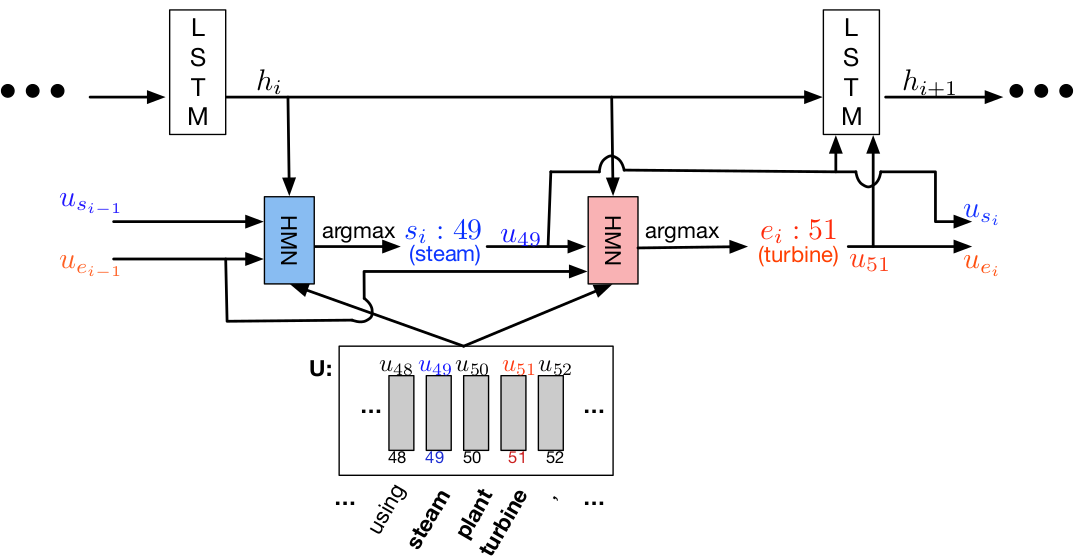
\includegraphics[width=1.0\linewidth]{dcn_dynamic_decoder.png}
    \caption{Dynamic decoder}
\end{figure}

$s_{i-1}$和$e_{i-1}$指的是第$i-1$次迭代所预测答案的起始位置和终止位置,
$u_{s_{i-1}},u_{e_{i-1}}$指的是第$i-1$次迭代所预测答案的起始位置和终止位置的那个单词在
协同注意力层输出矩阵$U$的向量表示。
\begin{gather}
s_i=\underset{t}{argmax}(\alpha_1,\cdots,\alpha_m)\notag \\
e_i=\underset{t}{argmax}(\beta_1,\cdots,\beta_m) \notag
\end{gather}
其中$\alpha_t$和$\beta_t$代表文章中第$t$个单词作为答案起始位置和终止位置的分数
$\alpha_t$和$\beta_t$的计算方式为:
\begin{gather}
    \alpha_t=\text{HMN}_{start}(u_t,h_i,u_{s_{i-1}},u_{e_{i-1}}) \notag \\
    h_i=\text{LSTM}_{dec}(h_{i-1},u_{s_{i-1}},u_{e_{i-1}}) \notag 
\end{gather}

$h_{i-1}$是第$i-1$次迭代时解码端的LSTM的隐藏状态,$u_t$是文章中第$t$个单词在$U$中的向量表示。
利用$h_{i-1},u_{s_{i-1}},u_{e_{i-1}}$计算出第$i$次迭代时LSTM的隐藏状态$h_i$,然后利用$h_i$以及
文章中每一个单词在$U$中的向量表示通过三层HMN网络计算出$\alpha$,$\alpha$的每一个值表示的就是文章中
每一个单词在第$i$次迭代作为答案起始位置的分数。

注意$\beta_t=\text{HMN}_{end}(u_t,h_i,u_{s_i},u_{e_{i-1}})$





\textbf{\kaishu \zihao{5} BiDirectional Attention Flow}
文献\upcite{Bidirectional attention flow for machine comprehension}提出一种双向注意力流模型,简称BiDAF。
首先在不同的语义粒度上表示文本,包括字符层面、单词层面、以及上下文层面。然后将问题或者段落的上下文表示送入到注意力流层。
注意力流层不同于之前流行的注意力机制
\begin{enumerate}
    \item 对于段落中每一个单词与问题计算得到的注意力结果,将它与前一层的这个单词的上下文表示连接然后流向后面的建模层
    \item 利用一种无记忆的机制,虽然类似于Bahdanau注意力\upcite{neural machine translation by jointly learning to align and translate},
对于段落的每一个时间步都会计算注意力,但是每一步计算的注意力是仅仅是关于段落和问题当前时刻的单词,与前面的时刻或后面的时刻计算的注意力都无关
    \item 不像之前的论文\upcite{Machine comprehension using match-lstm and answer pointer}仅仅
计算段落对问题的注意力,而忽视了问题对段落的注意力。
\end{enumerate}

之前的论文注意力机制大多借鉴于Bahdanau注意力\upcite{neural machine translation by jointly learning to align and translate},这种注意力运算机制的特点
就是说将段落中每一个单词的上下文表示和问题的上下文表示
做注意力的运算,计算的结果作为下一个单词做注意力计算的输入。但是这种计算方式显然前一时间步计算得到的注意力的结果会影响
下一时间步注意力的计算,也就是说这种注意力的计算方式在时间上来讲是动态的。而BiDAF在计算注意力时对于段落中
当前时间步的单词和问题计算注意力的结果不会参与下一时间步的单词计算注意力。这种机制简化了注意力的计算流程,使得注意力流层和后面的
建模层分隔开来,注意力流层会更加的专注于计算注意力,而且计算先前时间步计算的注意力出现偏差,也不会影响后面计算注意力。

具体的,输入给注意力流层的是上下文嵌入表示层的输出$C$和$Q$,其中$C\in R^{2d\times T}$是整个段落的上下文表示,
$Q\in R^{2d\times J}$是问题的上下文表示,$T$代表段落的长度,$J$代表问题的长度。
首先计算相似性矩阵$S$:
\begin{gather}
    S_{tj}=\alpha(C_{:t},Q_{:j}) \in R \notag \\ 
    \alpha(c,q)=w_{(S)}^T[c;q;c\circ q] \notag
\end{gather}

$\alpha$是编码两个向量$C$和$Q$相关性的函数,$w_{(S)}^T\in R^{6d}$是可训练的权重参数,$\circ$表示点乘。
$S\in R^{T\times J},S_{t:}\in R^{J},S_{:j}\in R_{T}$,每一行表示的段落中的一个单词对问题的相关度,每一列
表示的是问题的一个单词对整个段落的相关度。
接下来利用$S$计算两个方向的注意力,对于段落对问题的注意力C2Q,计算方式如下:
\begin{gather}
    a_t=softmax(S_{t:}) \notag\\
    \widetilde{Q}_{:t}=\sum_{j=1}^{J}a_{tj}Q_{:j}\notag
\end{gather}

$\widetilde{C}\in R^{2d\times T}$,Q2C的注意力的计算方式如下:
\begin{gather}
    b=softmax(max_{col}(S))\in R^T \notag \\
    \widetilde{q}=\sum_{t=1}^{T}b_tC_{:t} \notag 
\end{gather}
$S$的第$i$行的最大值那一列$j$表示的是段落中第$i$个单词和问题中第$j
$个单词之间的相关度最高,所以$\widetilde{q}$表示的就是段落中所有关于问题相关度最高的
单词的加权求和,这种计算方式略去了那些段落中关于问题不重要的单词。然后将$\widetilde{q}$在列的维度上
重复$T$次得到$\widetilde{Q}\in R^{2d\times T}$。

最后将计算的注意力结果$\widetilde{Q},\widetilde{C}$以及段落的上下文表示
按照$[P;\widetilde{P};p\circ\widetilde{P};P\circ\widetilde{Q}]\in R^{8d\times T}$这种方式连接,作为下一层建模层的输入。
可以看出计算出来的注意力流向了下一层,避免由于过早的把段落和文本概括为一个固定长度的向量导致信息的损失。

\textbf{\songti \zihao{5} R-Net}
文献\upcite{RNet}提出一种门控的自匹配网络。模型由四部分构成。

\begin{figure}[htbp]
    \centering
    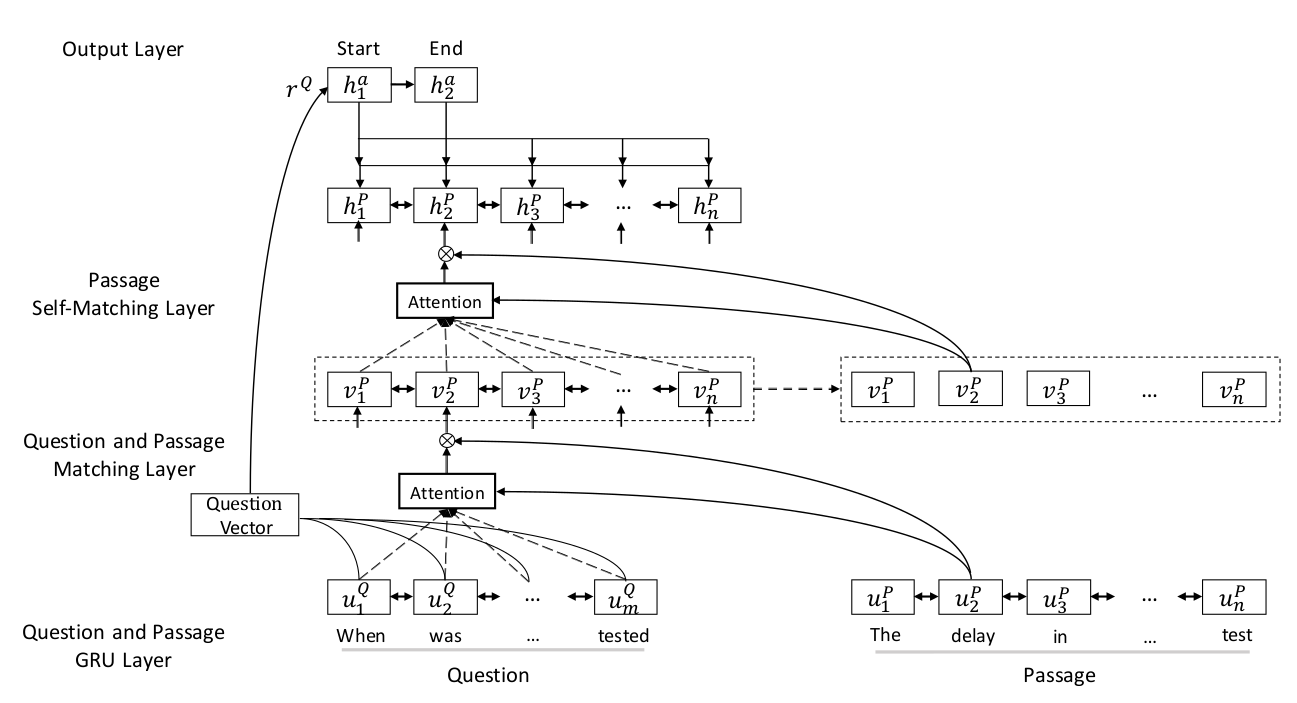
\includegraphics[width=1.0\linewidth]{rnet.png}
    \caption{Gated Self-Matching Networks structure overview.}
\end{figure}

第一部分利用双向GRU来编码文章和问题的词嵌入以及字符嵌入获得文章和问题中每一个单词的上下文表示,字符嵌入有助于解决那些未登录词典的词嵌入问题。
如图2所示,$u_1^Q,u_2^Q,\cdots,u_m^Q$表示经过BiGRU编码后的问题的上下文表示,$u_1^P,u_2^P,\cdots,u_n^P$表示文章的
上下文表示。

第二部分采用一种基于注意力的门控循环神经网络,这是基于注意力的循环神经网络的一种变体\upcite{neural machine translation by jointly learning to align and translate},
通过引入一个额外的门控单元放大那些在文章中与问题相关的部分的重要性,减小与问题无关的那部分的重要性。这种门控的思想
体现出一篇文章中只有其中一部分是与问题有关的。具体的计算方式如下:
\begin{gather}
    s_j^t=v^T\tanh(W_u^Qu_j^Q+W_u^Pu_t^P+W_v^Pv_{t-1}^P) \notag \\
    a_i^t=\exp(s_i^t)/\sum_{j=1}^{m}\exp(s_j^t)\notag \\
    c_t=\sum_{i=1}^{m}a_i^tu_i^Q \notag
\end{gather}
其中$u_j^Q$是问题的第$j$个单词的上下文表示,$u_t^P$是文章的第$t$个单词的上下文表示。$a_i^t$是
文章的第$t$个单词与问题的第$i$个单词之间的相关度。
$c_t$是将计算得到的注意力权重对整个问题加权求和得到的注意力结果。
$v_{t-1}^P$是当前层的循环神经网络上一时刻的隐藏状态。
\begin{gather}
    v_t^P=RNN(v_{t-1}^P,[u_t^P,c_t]^{*}) \notag \\
    [u_t^P,c_t]^{*}=g_t\circ [u_t^P,c_t] \notag \\
    g_t=\text{sigmoid}(W_g[u_t^P,c_t]) \notag 
\end{gather}
其中$g_t$为门控单元。

第三部分采用自匹配机制,虽然上一层的输出$v_1^P,v_2^P,\cdots,v_n^P$已经获得了关注问题的文章表示,但是一方面在SQuAD数据集中某些问题和文章
在语法和词汇上略有差异,另一方面循环神经网络实际上只能记忆有限的上下文信息,
从而导致答案中单词可能会忽视其周围单词的重要信息,
因此利用自匹配层对关注问题的文章表示做自注意力的计算。具体计算方式如下:
\begin{gather}
    s_j^t=v^T\tanh(W_v^Pv_j^P+W_v^{\widetilde{P}}v_t^P)\notag \\
    a_i^t=\exp(s_i^t)/\sum_{j=1}^{n}\exp(s_j^t)\notag \\
    c_t=\sum_{i=1}^{n}a_i^tv_i^P \notag \\    
    h_t^P=\text{BiRNN}(h_{t-1}^P,[v_t^P,c_t]^{*}) \notag \\
    [v_t^P,c_t]^{*}=g_t\circ [v_t^P,c_t] \notag \\
    g_t=\text{sigmoid}(W_g[v_t^P,c_t])\notag
\end{gather}\notag


第四部分是输出层,类似于Wang and Jiang\upcite{Machine comprehension using match-lstm and answer pointer}采用
Pointer Networks\upcite{Pointer Networks}来预测答案的起始位置和终止位置。在预测答案的起始位置时,输出层的初始状态
采用的是对问题中单词的上下文表示向量的加权求和。

\textbf{\zihao{5} QANet}
先前的模型大多使用循环神经网络来编码句子语义以及基于循环神经网络的注意力机制对文章和问题做交互。但是众所周知循环神经网络由于
序列式的特性使得训练是非常耗时的。另一方面循环神经网络由于梯度消失问题难以解决长距离依赖的情况。因此QANet\upcite{QANet}中完全
舍弃用循环神经网络作为编码器,而采用卷积神经网络与自注意力机制结合的方式再加入到transformers\upcite{Transformer}结
构中作为模型的编码器。值得一提的是虽然transformers结构已经被广泛的应用在各种NLP任务中,但是利用卷积与自注意机制的结合
是一种新的结构而且实验表明比单独的利用自注意力机制要高出2.7F1值。QANet的解码器结构与transformer的结构如图。
可以看出区别在于QANet中的编码器在输入自注意力层之前要经过几层卷积层。这里的卷积方式与传统的卷积方式不同,
采用的是深度可分离卷积\upcite{Deepwise Separable convolution}。这种卷积操作可以减少卷积层
中参数的数量。传统的卷积操作是在
每一个通道上利用卷积核同步卷积所有通道,而深度可分离卷积将传统的卷积步骤分为两个步骤。第一个步骤是
Depthwise卷积,也就是在这一步骤中每一个卷积核只负责一个通道,一个通道只由一个卷积核卷积,这样使得输入数据的特征在深度上是分离的。
第二个步骤是Pointwise卷积,将第一步输出数据在通道这一维度连接起来卷积。
完整的结构如图所示。

在输入嵌入层中一个单词的嵌入表示是词嵌入和字符嵌入的连接,其中词嵌入采用GloVe预训练的词向量\upcite{GloVe},字符嵌入采用\upcite{charCNN}
中的方式,利用卷积操作提取每一个单词的字符特征。然后将嵌入后的特征通过两层高速网络\upcite{Highway Network},输出的结果作为
嵌入编码层的输入。两个嵌入编码层的输出送入到注意力层做交互,这一层相似度矩阵的计算方式类似于BiDAF\upcite{Bidirectional attention flow for machine comprehension}
,在计算问题对文章的注意力时采用和DCN\upcite{Dynamic coattention networks for question answering}相似的计算方式,
即将文章对问题的注意力也同时考虑进去。注意力层的输出采用\upcite{Bidirectional attention flow for machine comprehension}
的思想,将文章对问题的注意力流向后面的层以减少过早加权和后的损失。然后将输出通过几层模型编码层,模型编码层后三层的输出分别作为
输入层的输入来分别的预测答案的起始位置的概率和终止位置的概率。输出层的设计是根据具体任务的,通过修改输出层,整个QANet也可以
用到其它类型的问答任务中。

数据增强
